\documentclass[conference]{IEEEtran}
\IEEEoverridecommandlockouts
% The preceding line is only needed to identify funding in the first footnote. If that is unneeded, please comment it out.
\usepackage{cite}
\usepackage{amsmath,amssymb,amsfonts}
\usepackage{csquotes}
\usepackage{hyperref}
\usepackage{algorithm}
\usepackage{algpseudocode}
\usepackage{graphicx}
\usepackage{textcomp}
\usepackage{xcolor}
\graphicspath{{./images/}}
\def\BibTeX{{\rm B\kern-.05em{\sc i\kern-.025em b}\kern-.08em
    T\kern-.1667em\lower.7ex\hbox{E}\kern-.125emX}}
\begin{document}

\title{Security of OpenSSL Tool}

\author{\IEEEauthorblockN{John Phillips}
\textit{johphill@mines.edu}\\
\and
\IEEEauthorblockN{2\textsuperscript{nd} Abhaya Shrestha}
\IEEEauthorblockA{\textit{ashrestha@mines.edu}}
\and
\IEEEauthorblockN{3\textsuperscript{rd} Joe Granmoe}
\IEEEauthorblockA{\textit{jgranmoe@mines.edu}}
\and
\IEEEauthorblockN{4\textsuperscript{th} Patrick Curran}
\IEEEauthorblockA{\textit{pcurran@mines.edu}}
\and
\IEEEauthorblockN{5\textsuperscript{th} Collin McDade}
\IEEEauthorblockA{\textit{collinmcdade@mines.edu}}
\and
\IEEEauthorblockN{6\textsuperscript{th} Noor Malik}
\IEEEauthorblockA{\textit{nmalik@mines.edu}}
}

\maketitle

\begin{abstract}
There have been small but catastrophic modifications to openssl in the
past\cite{1}\cite{2}\cite{5} that cause massive security problems and
in some cases exploits that can disclose private keys, or limit the
number of possible keys. We explore in depth one such instance, a
modification made to the OpenSSL package distributed in debian that
resulted in only 32,768 possible keys that could be generated. We also
explore similarities to heartbleed. Finally, we investigate methods
that have been put in place to prevent such bugs from happening in the
future.
\end{abstract}

\begin{IEEEkeywords}
OpenSSL, security vulnerability, debian
\end{IEEEkeywords}

\section{Introductionn}
\subsection{Background}
In 2008 a debian developer made a patch to openssl to fix valgrind
warnings\cite{2}\cite{3}. OpenSSL has a flexible system for generating
random numbers that uses an interface-like approach with functions
prefixed with \verb|RAND_*| delegating to a particular
implementation. Since this API was designed for cryptographic
applications, the random bytes generated need to not just satisfy
particular statistical properties, but be truly unpredictable. In order
to acheive this property, this particular random number generator
allows the user to add 'entropy' by feeding it buffers full of random
bytes. These bytes could be from \verb|/dev/urandom|, the user, or
somewhere else. When adding entropy in this way to the message
digest-based random API, an internal hash state is updated each time
with the random bytes given by the user. The hash state then can be
used to get random bytes back out of the system. 

In the OpenSSL code in 2006, there were several places where
uninitialized memory was deliberately read, in a couple ways. In order
to understand this, we mention two \verb|RAND_| functions:
\verb|RAND_add(const void *buf, int num, double entropy)| and
\verb|RAND_bytes(unsigned char *, int num)|. The first function,
\verb|RAND_add|, inputs the buffer \verb|buf| into the `pool' of
entropy, adding \verb|entropy| to the total entropy count. The buffer
is \verb|num| long.

With that understood, the first thing that the OpenSSL code would do
was call \verb|RAND_add| with a buffer that wasn't completely
initialized\cite{3}. For example, a function to initialize the random
library would read some bytes from a file into a buffer without
filling the buffer, and then call \verb|RAND_add| with that buffer and
it's full size as a parameter -- \emph{not} the number of bytes read
into the buffer. This ended up with uninitialized memory being used to
add to the entropy pool. One result of this deliberate over-reading of
buffers was that valgrind emitted errors coming from the default
implementation of the \verb|RAND_add| function, in \verb|md_rand.c|,
\verb|ssleay_rand_add|. Although that code itself was correct, it
would read uninitialized memory (which it was told to do by callers),
and cause a valgrind error to be emitted. This code was
\emph{critical} to the random number generator, and the line of code
generating the error in particular was essential to generating
entropy. To help understand this, we include a code excerpt that could
cause such an error (from \verb|crypto/rand/randfile.c|):

\begin{verbatim}
i = fread(buf, 1, n, in);
if (i <= 0) break;
/* even if n != i, use the full array */
RAND_add(buf, n, i);
\end{verbatim}

Note the comment -- \verb|buf| is \verb|n| long, but \verb|i| may be
less than \verb|n|. The end result is that the code called by
\verb|RAND_add| that actually reads and extracts entropy from
\verb|buf| will cause valgrind to emit a warning about reading from
uninitialized memory. However, if you commented out this code, you'd
also comment out the code that was actually extracting the entropy,
which is what happened.

The next cause of valgrind errors was also in
\verb|md_rand.c| -- there, the function \verb|ssleay_rand_bytes| would
update an internal hash with uninitialized memory -- the buffer that
was supposed to be a region to \emph{output} random bytes to was being
read from as a potential source of entropy. This code could be
commented out harmlessly, and probably shouldn't have been there in
the first place.

These two lines of code were the source of a complaint that first came
to the debian bug tracker\cite{2}. The debian developer quickly
spotted the `culprit' code -- that is, the lines of code that valgrind
identified as reading uninitialized memory -- but didn't know what it
did. Observing that commenting it out didn't cause anything to crash
or obviously function incorrectly, he asked on the openssl development
mailing list if it was okay to remove the two lines of code -- and got
the go-ahead (See Fig.\ref{email}).

Most linux distributions maintain small set of `patches' for each
package they distribute. These patches normally are designed to fix
critical bugs that haven't been fixed upstream or are in the process
of being fixed. So although the debian project doesn't maintain
OpenSSL, they could patch the particular version of OpenSSL
distributed by debian. And that was the solution arrived at in the bug
ticket and over email \cite{2}\cite{4}.

\begin{figure*}[!t]

\centering
\begin{displayquote}
\begin{verbatim}

List:       openssl-dev
Subject:    Re: Random number generator, uninitialised data and valgrind.
From:       Ulf_Möller <ulf () openssl ! org>
Date:       2006-05-01 22:34:12
Message-ID: 44568CE4.9020906 () openssl ! org
[Download RAW message or body]

Kurt Roeckx schrieb:
> What I currently see as best option is to actually comment out
> those 2 lines of code.  But I have no idea what effect this
> really has on the RNG.  The only effect I see is that the pool
> might receive less entropy.  But on the other hand, I'm not even
> sure how much entropy some unitialised data has.
>   
Not much. If it helps with debugging, I'm in favor of removing them. 
(However the last time I checked, valgrind reported thousands of bogus 
error messages. Has that situation gotten better?)
\end{verbatim}
\end{displayquote}

\caption{A reply to the email from the Debian Developer telling him to go ahead and modify the OpenSSL code.\cite{4}}
\label{email}
\end{figure*}


The debian developer then applied the patch and distributed the debian
version of OpenSSL with this critical vulnerability built in. One of
the two lines commented out was in fact essential to adding entropy to
the system, and with it commented out, none of the calls to
\verb|RAND_add| actually did anything. This vulnerability was
distributed to all users of debian from 2006 to 2008\cite{1}. During
that entire time, any code using the random number generator could
only really have 32,768 possible outputs from the random number
generator. Examples of affected functions included TLS modules and SSH
key generation -- actually, anything that generated RSA keys was
vulnerable.

\subsection{Motivation and Goal}

Because of the infamous vulerability that OpenSSL had in the past,
we aim to understand one of the vulnerabilities
of the past (2008 OpenSSL vulnerability), research OpenSSL
methods in place to prevent vulnerable code from being
shipped, and experiment on the library by seeing if
the vulnerability of the past could be detected with methods
they have set up in the present (particularly functional, and fuzz testing).

\section{Recreating the 2008 bug}

In order to gain a better understanding of exactly how the bug worked,
and how easy (or difficult) it would be to exploit such a flaw, we
used virtual machines and code from the 2008 era to see what
exploiting the vulnerability might look like. The basic idea was to
create two virtual machines. One would be the exploited machine -- a
stand-in for a server on the Internet or other network that had an
open SSH port that was believed to be secure. The other machine would
try to access the target server over SSH by repeatedly generating
trial keys until it was able to successfully get in. Although this is
not as simple as just writing code to guess the key and compare two
files, it is arguably a more realistic demonstration of how exploits
really work, and a better way of understanding them, putting the
`applied' in `applied cryptography'.

\subsection{Code modifications}
First, we created two different versions of the OpenSSL code. The
first one had the two lines that the debian developer asked about on
the OpenSSL mailling list commented out (see \cite{4}), and nothing
more. It was a re-creation of what existed in the debian project from
2006-2008. We looked for the exact code (for example, a .deb binary
distribution, or the actual patchsets applied to the OpenSSL project)
on the Internet but were unable to find it (links pointing to the
patches were all dead, possibly in a deliberate attempt by debian to prevent
anyone accidentally using the code again).

The next branch of the OpenSSL code was similar to the first except it
had a way to manually set the only real source of variablility left to
the random number generator -- the PID (process ID). We did this by
replacing calls to \verb|getpid()| in \verb|md_rand.c| to references
to a static variable in \verb|md_rand.c| called \verb|fake_pid|. We
also introduced a globally-visible function called
\verb|RAND_exploit_set_pid()|, to allow client code to set the PID.


\subsection{Virtual machine setup}
We built two virtual machines based on debian 5. The machines were
connected to a single virtual switch, and had static IPs assigned. On
one virtual machine, we built and installed the re-created
debian-distributed OpenSSL. We used \verb|ssh-keygen| to create and
authorize a key as an authorized SSH key on that host.

On the other (attacker) machine, we used a program derived from
\verb|ssh-keygen| to try to SSH to the target machine with a given PID
seed. That program then was repeatedly invoked by another script that
iterated over all possible PIDs, from 1 to 32,768 (in 2008 that was
the number of possible PIDs).

The results were as expected -- the attacker machine was able to
generate the public/private key pair of the target machine within
fifteen to twenty minutes. On a fresh boot, because there haven't been
as many processes run, it takes only about five minutes.

\subsection{Running the exploit}
Since the virtual machines are connected over a virtual network, to
run the exploit, we simply boot them and run a script on the attacker
machine that will eventually break the key of the target machine. The
attacker script will then write the public/private key pair to a
file. See Appendix A for details.

\subsection{Alternative approaches}

\section{Similarities to Heartbleed}
The debian bug bears certain similarities to another bug that occurred
in 2014 -- Heartbleed\cite{4}. Both bugs compromised private keys, and
both were not the result of any protocol design errors, cryptanalytic
breakthroughs that allowed algorithms to be broken, or any other issue
commonly learned about in a cryptography class. Instead, both errors
were the result of human error. Simple, and (in hindsight) rather
obvious bugs made their way into OpenSSL packages that were
distributed to an untold number of machines.

With heartbleed, the issue was simply a missing boundary
check\cite{16}. First, code was added to allow for an extension to the
SSL/TLS protocol that sent `heartbeats'. This allows for the SSL
connection to be kept alive \cite{16}. The fix was only a few lines of
code\cite{17}.

Although one bug was an alteration of working code and the other was
adding a buggy feature, the critical piece of both involved reading
past array bounds. In the debian bug, a call to \verb|MD_Update()| was
uninitialized memory and caused a valgrind error, which triggered the
faulty fix. In Heartbleed, a boundary check was not made that allowed
attackers to read uninitialized memory.

This raises the question of how, if possible, to catch such simple
implementation errors? Possible solutions are using CI/CD and a good
automated test suite that has high code coverage and covers
edge-cases. We can see that both bugs would have been stopped if:

\begin{itemize}
  \item The OpenSSL library was designed from the start to use static
    and dynamic analysis tools like valgrind (no false positives as in
    the case of the debian bug, and possible warnings in the case of
    Heartbleed), sanitizers, and static code analysis tools like \verb|cppcheck|.
  \item The OpenSSL library had high-coverage functional testing, and
    a test suite that was automatically run before anyone distributed
    a new or modified OpenSSL. This can be accomplished with compiler
    tools that generate test coverage data like \verb|gcov| and
    \verb|lcov|.
\end{itemize}

In the next section we examine if this situation has improved.

\section{Investigating the current code}

\subsection{Architectural differences}
In the current code, the old \verb|md_rand.c| has been removed. It was
renamed to \verb|ossl_rand.c| in June of 2017 \cite{13}, and removed
in August, to be replaced by the DRBG api\cite{14}. The DRBG api is
based on the NIST standard NIST SP 800-90A, for `Deterministic Random
Number Generator' \cite{10}\cite{15}.

The current code also has a much greater unit test coverage in the
\verb|test/| directory. Where previously there were a few very simple
and esoteric tests based on shell scripts to check basic correctness
-- for example, the file \verb|test/trsa| is a shell script that tests
if the \verb|openssl rsa| command can convert RSA keys between
different plaintext formats -- there are now much more comprehensive
tests that test the DRBG for duplicate results. If these had been in
place before the debian key bug, perhaps it never would have happened.

\subsection{Code quality improvements}
We were able to demonstrate that the valgrind errors observed in
\cite{2} actually were visible in the unit tests themselves in the old
OpenSSL (version \verb|0.9.7e|), when running the test \verb|exptest|
in the \verb|test| directory (see Appendix A for details). Not only
that but the OpenSSL code in general from that era was littered with
valgrind errors, with valgrind not counting more errors on some tests
because there were so many. Using the \verb|lcov| tool, code coverage
was measured at around 41.7\%, covered in Appendix C (see Table
\ref{branches-coverage} also). This left lots of room for bugs to slip
through, and none of the tests failed on the branch that contained the
debian modifications -- so the debian developer had no way to test his
work other than trust in the mailing list.

The current state of the code (the \verb|master| branch as of March
25, 2022) is certainly better, although perhaps by not as much as
would be ideal. We ran the functional test suite in the \verb|test/|
directory to see code coverage, using the same method for
\verb|0.9.7e|. Code coverage improved to a total of 65.1\% of lines (see
Appendix C for how to get this information for yourself). We noticed
that some of the implementation files for the DRBG, in
\verb|providers/implementations/rands/drbg.c| had many uncovered
edge-cases. Although the code may work now, uncovered edge cases in
the test suite mean that the code isn't defended from potential future
changes like the one made by the debian developer in 2006.

We did confirm that similar alternations to the DRBG code to the ones
made in 2006 by the debian developer \emph{did} cause unit tests to
fail in the newer test suite (version 3.0.0), see Appendix B for more.

Although code coverage and the state of the unit tests has improved,
65.1\% unit test coverage leaves a lot to be desired. In a
security-critical library, the 35\% of untested code could easily have
devastating un-tested flaws, that could wait for years before being
found.

  Next, we ran fuzz testing with their specified directions to see if
it would detect any of those changes. Particularly, we ran AFL 
library. The library timed out on two
of the fuzzers (\verb|bignum| and \verb|asn1|) and failed. When
we extend the timeout of afl fuzzer with \verb|-t 5000| flag for
those two fuzzers and it did
not timeout anymore. All of the other
fuzzers did not timeout and fail. These two fuzzers only failed due to timeout and not because they
detected a vulnerability. Therefore, we conclude that fuzz testing were unable to detect
the alterations made to DRBG code. For more details, we further explain
our process on Appendix B.

\section{Processes in the OpenSSL project in place to prevent further exploits}

Exploring OpenSSL project contribution process, we looked into what it
takes to be a committer in their repo, whether they have any kind of
automated checking in place (CI or Continuous Integration), and what
their approval process looks like.

Before we delve into the process, we need to define a few terms from
their glossary.

\begin{enumerate}
\item \textbf{OMC (OpenSSL Management Committee)}: they oversee all
  managerial and administrative aspects of the project. They are the
  final authority for the project\cite{6}

\item \textbf{OTC (OpenSSL Technical Committee)}: they oversee all
  technical aspects of the project\cite{6}.

\end{enumerate}

\subsection{What it takes to be a Commiter of OpenSSL?}

To become a committer, one has to be granted access by the OMC on the
recommendation of OTC\cite{7}. This access can be withdrawn at any
time by a vote of the OMC\cite{8}. In order to maintain their
committer status, a commiter must have authored or reviewed at least
one commit within the previous two calendar quarters\cite{8}.

They expect committers to be experts in some part of low-level crypto
library as well as generalists who contribute to all areas of the
codebase\cite{7}. Committers are expected to oversee the health of the
project: fixing bugs, addressing open issues, reviewing contributions,
and improving tests and documentation\cite{7}. According to OpenSSL,
to be a commiter, one can start by contributing code, reading code
style, and getting to know build and test system\cite{7}. In short,
anyone can be a commiter as long as they are granted access by OMC on
recommendation of OTC.  Their contributions can range from small
documentation fixes, spelling errors, to large code base
contributions.

\subsection{What automation checks does OpenSSL have to ensure code safety?}

Based off of their glossary, we were able to understand that OpenSSL
uses Continuous Integration which is a suite of tests and checks that
are run on every pull request, commit on a daily basis. Some of their
tests include functional tests, performance testing, and fuzz
testing\cite{9}. These kinds of tests are described as follows.

\begin{enumerate}
\item \textbf{Functional Tests}: given a set of inputs, it
  will produce a correct set of outputs\cite{9}.

\item \textbf{Performance Tests}: These tests test performance, and
  will be performed automatically via CI on a regular basis for
  certain components. Examples include:

  \begin{itemize}
  \item Individual algorithm performance operating over different
    input sizes
  \item SSL/TLS handshake time over multiple handshakes and for
    different protocol versions and resumption/non-resumption
    handshake.
  \end{itemize}\cite{9}.

\item \textbf{Fuzz Tests}: Systematic methodology that is used to find
  buffer overruns (remote execution); unhandled exceptions, read
  access violations (AVs), and thread hangs (permanent
  denial-of-service), and memory spikes (temporary
  denial-of-service)\cite{10}.

\end{enumerate}

According to their testing policy, a pull request does not require testing
if the changes are as follows\cite{9}.

\begin{itemize}
\item Documentation (including CHANGES/NEWS file changes)
\item The test suite
\item perl utilities
\item include files
\item build system
\item demos
\end{itemize}

Additionally, they recommend adding fuzz testing when implementing
significant new functional tests or at least consider adding fuzz
testing when refactoring to check all corner cases are
covered\cite{9}.  OpenSSL particulary uses either LibFuzzer or AFL to
do fuzz testing \cite{11}. While performance tests improve the
functionality of OpenSSL, fuzz testing and functional testing helped
us ensure that OpenSSL codebase is at least sanity checked. Fuzz tests
especially help since they are basically dynamic analysis detection
for any vulnerabilities or bugs in the codebase.

\subsection{What does their approval and code review process look like?}
    OpenSSL approval and code reviews process are as follows.

    \begin{itemize}
        \item OpenSSL pull requests are reviewed and approved by at
          least two committers, one of whom must be an OTC
          member. Neither of the reviewers can be the author of the
          submission\cite{7}.  The only exception to this policy is during
          the release process when the author's review does not count
          towards the two needed reviews for the automated release
          process and NEWS and CHANGES file updates\cite{7}.

        \item In case two committers make a joint submission, they can
          review each other's code, but not their own. Additionally, a
          third reviewer will be required\cite{7}.

        \item An OMC/OTC member may apply a needs OMC decision label
          to a submission which can hold the submission. This hold may
          only be removed by OTC/OMC member who put the hold or the
          OTC/OMC\cite{7}.

        \item Approved submission (besides automated release process
          and NEWS and CHANGES file updates) will only be applied
          after 24-hour delay from approval. An exception to the delay
          exists for build and test breakage fix approvals which will
          be flagged with the severity: urgent label\cite{7}.
    \end{itemize}

    Additionally, on their commit workflow, their public github
    repository is just a mirror and pulls from the real repo where
    only committers have access\cite{7} (When someone becomes a
    committer, OpenSSL will send instructions to get commit access to
    the repository\cite{7}).  Finally, they also have strict
    documentation design process whenever minor or major code changes
    the design, and changes to existing public API functions and data
    are forbidden \cite{9}. However, they encourage a new API call to
    be implemented if need be as a minor release \cite{9}. From this
    information, we can definitely tell that today it is difficult to
    be able to commit anything without prior granted permissions and
    approval to OpenSSL. Futhermore, even if changes were to occur,
    they always run their automation process to detect any defects or
    vulnerabilities with their test suites which is very assuring for
    a user of OpenSSL.
    \\

    \quad However, there are still chances that a defect or
    vulnerability could be shipped out. Particularly, when they
    suggested that refactors do not need a test but recommend Fuzz
    testing to cover edge cases. In the refactor case, there is a
    possibility that the committer misses an edge case in fuzz testing
    and creates a bug or vulnerability.  Another challenge of a
    cryptographic tool such as OpenSSL is that professionals do not
    know how to test for security. An algorithm implementation is only
    secure if an attacker cannot decipher or find vulnerabilities to
    exploit for the algorithm. Futhermore, Fuzz tests are basically
    just shooting in the dark and hoping to find a vulnerability
    before the adversary finds it.  Nonetheless, we have to say their
    process for who gets to commit code to the master is solid;
    however, there is no assurance that a vulnerability will not be
    shipped out.  The best we could do is hope that the code review
    and automation process detects a defect or vulerability and
    prevents it from being shipped out.

\section{Conclusion}
To understand how a vulnerability like the 2008 debian OpenSSL bug
happens and can be exploited, we read the code from that period and
built an exploit that would be able to unlock affected machines using
SSH keys.

Next, we did a survey of the state of the code then and now to see if
the introduction of such code was due to incompetence on the debian
developer's part, or an understandable error that no automated tools
were in place to catch. We concluded that there was no easy way to
tell if the code modification would adversely affect the security of
the library, and that, furthermore, the debian developer was given the
go-ahead.

The current state of the code is much better however, having more
thorough unit-testing coverage that can catch more accidental errors
made by OpenSSL developers or package distributors. Furthermore, the
current implementation of OpenSSL's random number generator is based
on a specification and is therefore much easier to reason about.

We concluded that the security of the OpenSSL tool has increased
substantially since the 2008 debian OpenSSL bug was caught, the
heartbleed vulnerability notwithstanding.
    
\begin{thebibliography}{00}
\bibitem{1} D. Winter, ``Debian's openssl disaster: Isotoma: Our blog'', Isotoma, 14-May-2008 (Online), 
  \url{https://isotoma.com/blog/2008/05/14/debians-openssl-disaster/} (Accessed: 11-May-2022). 
\bibitem{2} R. Kettlewell, ``Debian bug report logs - \#363516 valgrind-clean the RNG'', bugs.debian.org, 19-Apr-2006 (Online), 
  \url{https://bugs.debian.org/cgi-bin/bugreport.cgi?bug=363516} (Accessed: 11-May-2022). 
\bibitem{3} R. Cox, ``Lessons from the Debian/OpenSSL fiasco'', research!rsc, 21-May-2008 (Online), 
  \url{https://research.swtch.com/openssl} (Accessed: 11-May-2022). 
\bibitem{4} U. Möller, ``re: Random number generator, uninitialised data and valgrind.'', marc.info, 
  \url{https://marc.info/?l=openssl-dev&amp;m=114652287210110&amp;w=2} (Accessed: 11-May-2022). 
\bibitem{5} I. Synopsys, ``The heartbleed bug'', Heartbleed Bug,
  \url{https://heartbleed.com/} (Accessed: 11-May-2022). 
\bibitem{6} OpenSSL, ``Glossary of OpenSSL terms'', openssl.org,
  \url{https://www.openssl.org/policies/glossary.html}(accessed Apr. 20, 2022).
\bibitem{7} OpenSSL, ``Policy for OpenSSL Committers'', openssl.org,
  \url{https://www.openssl.org/policies/general/committer-policy.html}(accessed Apr. 20, 2022).
\bibitem{8} OpenSSL, ``OpenSSL Bylaws'', opessl.org, 
  \url{https://www.openssl.org/policies/omc-bylaws.html}(accessed Apr. 20, 2022).
\bibitem{9} OpenSSL, ``OpenSSL Technical Policies'', openssl.org,
  \url{https://www.openssl.org/policies/technical/}(accessed Apr. 20, 2022).
\bibitem{10} John Neystadt, ``Automated Penetration Testing with White-Box Fuzzing'', docs.microsoft.com,
  \url{https://docs.microsoft.com/en-us/previous-versions/software-testing/cc162782(v=msdn.10)?redirectedfrom=MSDN}
  (accessed Apr. 20, 2022).
\bibitem{11} OpenSSL, ``Fuzzing OpenSSL'', github.com,
  \url{https://github.com/openssl/openssl/tree/master/fuzz}(accessed Apr. 20, 2022).
\bibitem{12} ``Recommendation for Random Number Generation Using
  Deterministic Random Bit Generators'', revision 1,
  \url{https://doi.org/10.6028/NIST.SP.800-90Ar1}, June 2015.

\bibitem{13} Salz, Richard, OpenSSL Source code, commit da8fc25a989cf4f4d26d626a85477e8a9282da12, June, 2017.

\bibitem{14} Salz, Richard, OpenSSL Source code, commit 75e2c877650444fb829547bdb58d46eb1297bc1a, August 2017.

\bibitem{15} OpenSSL Project, ``\verb|RAND_DRBG|'', OpenSSL
  Documentation,
  \url{https://www.openssl.org/docs/man1.1.1/man7/RAND_DRBG.html}

\bibitem{16} Rubenking, Neil, ``Heartbleed: How It Works'', \emph{PCMAG}, \url{https://www.pcmag.com/news/heartbleed-how-it-works}, (accessed May 10, 2022).

\bibitem{17} Henson, Stephen, OpenSSL SOurce code, commit 96db9023b881d7cd9f379b0c154650d6c108e9a3, April 2014.

\end{thebibliography}

\appendices{}
\section{Building and running the exploit}
For the project we built a git repository found at
\url{https://github.com/john-w-phillips/crypto-project}. The file
\verb|README.md| there contains detailed information about running the
exploit but we include some here as a general overview.

First, we'll cover alterations we made to the OpenSSL code.

\subsection{The OpenSSL Repository}
We added a subrepository in the \verb|openssl| folder that contains a
mirror of the OpenSSL git repository. From there we were able to
analyze the state of OpenSSL code from several points in time. To make
things easy we checked out these points in time on branches. See
Table \ref{branches} for details.

\begin{table*}[!t]
  \centering
  \begin{tabular}{|l|l|}
    \hline
    Branch name & Function \\ \hline
    \verb|debian-mod-point| & The code that was distributed by Debian starting in 2006 \\ \hline
    \verb|hacked-ssl-for-running-exploit| & Code we used to run the exploit. \\ \hline
    \verb|openssl-broken-tests-demo| & Code in version 3.0 deliberately broken to demonstrate that test coverage improved. \\ \hline
    \verb|master| & Current OpenSSL code \\ \hline
  \end{tabular}
  \caption{Branches in the openssl subrepository and their function.}
  \label{branches}
\end{table*}

To build this code you can read the \verb|INSTALL| file. Basically the
steps are as follows:

\begin{verbatim}
$ ./config shared
$ make -j
$ make install # if needed.
\end{verbatim}

This will install ssl libraries and headers in \verb|/usr/local|. If
SSL is already installed, you may need to modify
\verb|LD_LIBRARY_PATH| to link existing executables against the
compiled SSL libraries.  With OpenSSL built we can do several things
with it.

\subsection{The OpenSSH Repository}
One way to take advantage of the vulnerability in question was to
attack SSH keys. We decided to demonstrate how such an attack would
work. To do so, we used the standard \verb|ssh-keygen| on the target
box (one that came with the debian distribution -- ssh had no built-in
vulnerability other than its dependency on OpenSSL), but a heavily
modified version of this program on the attacker box to iteratively
generate the potential SSH keys that a machine with the flawed code
could have, and try them out, using a brute-force style attack. There
are two components to this: \verb|ssh-exploit-driver.bash| and
\verb|ssh-keyexploit.c|. The \verb|ssh-exploit-driver.bash| script
takes an IP address and iterates over all possible PID seeds,
1-32,768, and runs \verb|ssh-keyexploit.c| with each one.

See Algorithm \ref{ssh-keyexploit} for how \verb|ssh-keyexploit.c|
works.

\begin{algorithm}
  \caption{SSH key exploit}\label{ssh-keyexploit}

  \begin{algorithmic}[1]
    \Procedure{exploit}{$IP,PID$}
    \State Set the PID in the OpenSSL modified library from $PID$
    \State $\mathrm{RSA}_{\mathrm{PU}}, \mathrm{RSA}_{\mathrm{PR}} \gets$ Modified OpenSSL generated key with $PID$ as only source of variability.
    \State $success \gets$ Try to SSH into host given by $IP$ with $\mathrm{RSA}_{\mathrm{PR}}$.
    \If{$success$}
    \State Report success
    \Else
    \State Report Failure
    \EndIf
    \EndProcedure
  \end{algorithmic}
\end{algorithm}

We run the exploit by running the script with the IP address of the
target machine. With the provided virtual machines, this would look like this:

\begin{verbatim}
$ ./ssh-exploit-driver.bash 10.10.1.5
\end{verbatim}

Eventually on the attacker machine you will get the output seen in
Fig.\ref{successfulexploit}.

\begin{figure*}
  \centering
  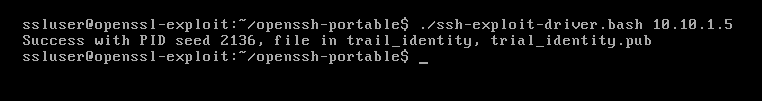
\includegraphics[width=4in]{images/SuccessfulExploit}
  \caption{Console output of successful exploit}
  \label{successfulexploit}
\end{figure*}

You can then SSH to the target machine with the \verb|trial_identity|
file.


\section{Measuring effects of unit and fuzz tests}

As part of our analysis we wanted to see if the new unit test
framework (since 2008) would catch the kind of error the debian
developer introduced in 2006. Since the new random number generator,
DRBG, is specification-based and much less arbitrary, this isn't an
apples-to-apples comparison.

First, we tried running the old test suite to see if it would have
caught the debian-introduced bug, or if the debian developer was
simply negligent. In that version of OpenSSL, tests are run with the
comand \verb|make alltests| in the \verb|test| directory.  No tests
failed -- so the automated test suite didn't catch this modification.

Since we can't comment out the same lines in newer OpenSSL versions,
we decided to find an area of code that's critical to updating the
entropy of the DRBG random number generator. The DRBG random number
generator, as specified in \cite{12}, has a few different sources of
potential entropy to be mixed in to the `pool'. The secure source of
entropy, which must remain secret, is only used while seeding the
DRBG. The critical activity here occurs when that entropy is hashed
into the internal state of the DRBG. This occurs in \verb|drbg_hash.c|
in the \verb|hash_df| function, which is an implementation of
\textbf{Hash\_df} as specified in \cite{12}. After that, users also
have the option to mix (untrusted) entropy into the random number
generation process using `additional input' strings, which are
optional.

In order to see if the debian bug could happen again today with a
similar error, we commented out all lines of code that updated the
internal hash state of the hash-based DRBG, and ran unit tests to see
if this caused them to fail. To run unit tests, complete the basic
build process as described above and then type:

\begin{verbatim}
make test
\end{verbatim}

We determined that this error is caught, see the error message in
Fig.\ref{testfailure} that was the output of \verb|make test|.

\begin{figure*}[!t]

\centering
\begin{verbatim}
30-test_evp.t ...................... 19/? 
        # INFO:  @ test/testutil/stanza.c:21
        # Reading ../../test/recipes/30-test_evp_data/evprand.txt
        # INFO:  @ test/testutil/stanza.c:122
        # Starting "CAVP Large Seed" tests at line 17
        # INFO:  @ test/testutil/stanza.c:122
        # Starting "CTR DRBG No Reseed Tests (from NIST test vectors)" tests at line 34
        # INFO:  @ test/testutil/stanza.c:122
        # Starting "Hash DRBG No Reseed Tests (from NIST test vectors)" tests at line 6324
        # ERROR: (memory) 'got == item->output' failed @ test/evp_test.c:2599
        # --- got
        # +++ item->output
        # 0000:-919f858c8a03c8a6 7eb2a0f54d2a409a 5b4bb94ecaefeefe b1c9b31ac049d127
        # 0000:+0e28130fa5ca11ed d3293ca26fdb8ae1 810611f78715082e d3841e7486f16677
        #       ^^^^^^^^^^^^^^^^ ^^^^^^^^^^^^^^^^ ^^^^^^^^^^^^^^^^ ^^^^^^^^^^^^^^^^
        # 0020:-7ccfeecc0a2a85df 16d23b14ad21b87a 5ffd238e2ae34a41 59a3fb4f39377975
        # 0020:+b28e33ffe0b93d98 ba57ba358c1343ab 2a26b4eb7940f5bc 639384641ee80a25
        #       ^^^^^^^^^^^^^^^^ ^^^^^^^^^^^^^^^^ ^^^^^^^^^^^^^^^^ ^^^^^^^^^^^^^^^^
        # 0040:-15f91a5edeca7aa1 7d30428bf31cd0dd
        # 0040:+140331076268bd1c e702ad534dda0ed8
\end{verbatim}
\caption{A test failure, catching the modified DRBG. This didn't happen in the earlier OpenSSL.}
\label{testfailure}  
\end{figure*}

  For the fuzz tests, OpenSSL recommended using LibFuzzer or AFL.
We tried AFL following their instructions on the README at \url{https://github.com/openssl/openssl/blob/master/fuzz/README.md}.
Their fuzzers run infinitely until the tester kills
the program or fuzzer detects a crash
according to the instructions; therefore, we only
timed the fuzzers for 3 minutes until it crashed or caught something. With
AFL, we were able to successfully run all
fuzzers without any problems, but 
found timeout on \verb|bignum| and \verb|asn1|. We wanted
to further investigate the cause of the timeout. Therefore, we increased 
the timeout to 5 seconds with the command 

\verb|afl-fuzz -t 5000 -i fuzz/corpora/$FUZZER|
\verb|  -o fuzz/corpora/$FUZZER/out fuzz/$FUZZER|
where \verb|$FUZZER| is \verb|bignum| or \verb|asn1|, it was successfully able to execute those tests
as we saw the statistics screen on Figure 4 (asn1 example, but same screen was shown
when using bignum). 
  
  In conclusion, we would have to say the fuzz testing were not able to detect any
vulnerabilities. The results are show in Figure 3 for
the timeout failure, and Figure 4 when timeout
gets updated with \verb|-t 5000| option run with AFL (this test in particular ran for almost two
hours before we decided to conclude nothing was found).
\begin{figure}[h]
  \caption{AFL test timeout for asn1 fuzzer}
  \centering
  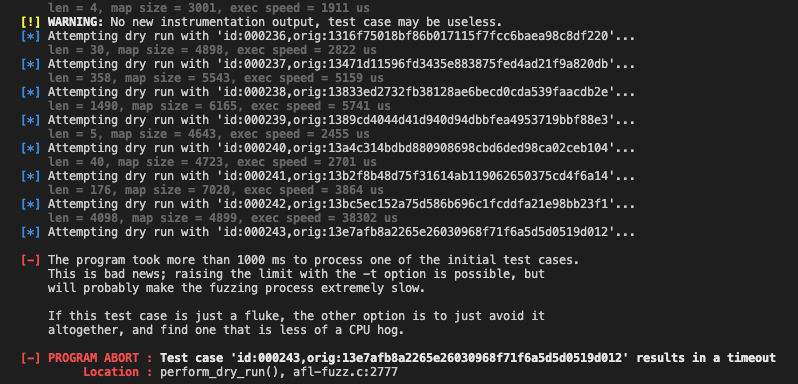
\includegraphics[scale=0.3]{asn1-fuzz-failure}
\end{figure}
\begin{figure}[h]
  \caption{AFL test with timeout increased}
  \centering
  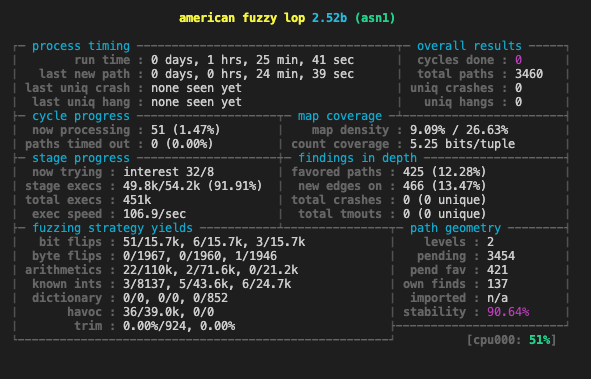
\includegraphics[scale=0.3]{asn1-fuzz-timeout}
\end{figure}

\section{Measuring test coverage}
We also wanted to measure test coverage. Test coverage is a way of
measuring how much code actually gets executed during a test run. You
can get two basic kinds of measurements: percentage of lines executed,
or percentage of functions. We focus on percentage of lines, since
percentage of functions can leave out edge cases.

To measure code coverage, we used the \verb|--coverage| flag with GCC,
and the \verb|view-test-coverage.sh| script which generates a
graphical report of test coverage viewable in a web browser. See
Fig.\ref{coveragedemo} for an example of what the coverage looks
like. The details of compiling for coverage testing varied. For the
\verb|master| branch, the following commands worked:

\begin{verbatim}
./config CFLAGS="--coverage -fprofile-arcs" \
         LDFLAGS="-fprofile-arcs -lgcov"
make -j
make test
../view-coverage.sh
\end{verbatim}

However, for the \verb|debian-mod-point| branch, a slightly different
set of commands was needed:

\begin{verbatim}
./config -lgcov -fprofile-arcs \
         -ftest-coverage shared
make -j
make test
../view-coverage.sh
\end{verbatim}

See Table \ref{branches-coverage} for our results.

\begin{figure*}[!t]
  \noindent\makebox[\textwidth]{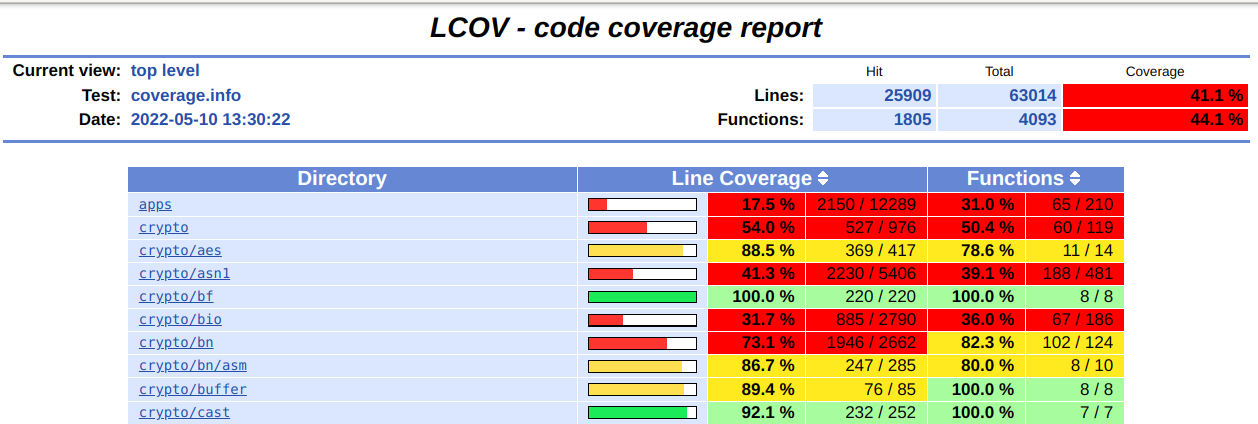
\includegraphics[width=\paperwidth]{images/TestCoverageDebianModPoint}}
  \caption{Example test coverage output using the lcov tool}
  \label{coveragedemo}  
\end{figure*}

\begin{table*}[!t]
  \centering
  \begin{tabular}{|l|l|}
    \hline
    Branch name & Coverage \%  (by line)\\ \hline
    \verb|debian-mod-point| & 41.7\% \\ \hline
    \verb|master (version 3) | & 65.1\% \\ \hline
  \end{tabular}
  \caption{Branches in the openssl subrepository and test coverage.}
  \label{branches-coverage}
\end{table*}
\end{document}
